 \iffalse
\let\negmedspace\undefined
\let\negthickspace\undefined
\documentclass[journal,12pt,twocolumn]{IEEEtran}
\usepackage{amssymb}
\usepackage{cite}
\usepackage{amsmath,amssymb,amsfonts,amsthm}
\usepackage{algorithmic}
\usepackage{graphicx}
\usepackage{textcomp}
\usepackage{xcolor}
\usepackage{txfonts}
\usepackage{listings}
\usepackage{enumitem}
\usepackage{mathtools}
\usepackage{gensymb}
\usepackage{comment}
\usepackage[breaklinks=true]{hyperref}
\usepackage{tkz-euclide} 
\usepackage{listings}
\usepackage{gvv}                                        
\def\inputGnumericTable{}                                 
\usepackage[latin1]{inputenc}                                
\usepackage{color}                                            
\usepackage{array}                                            
\usepackage{longtable}                                       
\usepackage{calc}                                             
\usepackage{multirow}                                         
\usepackage{hhline}                                           
\usepackage{ifthen}                                           
\usepackage{lscape}
\usepackage{pgfplots}
\newtheorem{theorem}{Theorem}[section]
\newtheorem{problem}{Problem}
\newtheorem{proposition}{Proposition}[section]
\newtheorem{lemma}{Lemma}[section]
\newtheorem{corollary}[theorem]{Corollary}
\newtheorem{example}{Example}[section]
\newtheorem{definition}[problem]{Definition}
\newcommand{\BEQA}{\begin{eqnarray}}
\newcommand{\EEQA}{\end{eqnarray}}
\newcommand{\define}{\stackrel{\triangle}{=}}
\theoremstyle{remark}
\newtheorem{rem}{Remark}
\begin{document}

\bibliographystyle{IEEEtran}
\vspace{3cm}

\title{NCERT Discrete-11.9.4-5}
\author{EE22BTECH11004 - Allu Lohith}

\maketitle
\newpage
\bigskip


 Find the sum of n terms of this sequence:$$5^2+6^2+7^2...+20^2$$  
\solution
\fi
\begin{table}[h!]
\centering
\renewcommand{\arraystretch}{2}
\begin{tabular}{|c|p{4cm}|c|}
\hline 
\setlength{\tabcolsep}{1pt}
\textbf{Parameter}  &\textbf{Description} &\textbf{Formulae/Value} \\
\hline
n & Iteration number starting from zero till 15 & - \\
\hline
$x\brak n$ & General term of the sequence from $n=0$ to $n=15$ &$\brak{n+5}^2$  u\brak n\\
\hline
$x\brak 0$ & First term of the sequence & 5 \\
\hline
\end{tabular}

\vspace{0.5cm}
\caption{\normalsize Parameters}
\end{table}
The standard $z$ transforms,
\begin{align}
    u \brak n &\stackrel{z}{\longleftrightarrow} \frac{1}{1-z^{-1}}, \abs z >1\\
   n u\brak n &\stackrel{z}{\longleftrightarrow} \frac{z^{-1}}{\brak{1-z^{-1}}^2}, \abs z >1\\
   n^2 u\brak n &\stackrel{z}{\longleftrightarrow} \frac{z^{-1}\brak{1+z^{-1}}}{\brak{1-z^{-1}}^3}, \abs z >1
\end{align}
As 
\begin{align}
    x\brak n = \brak{n^2+10n+25}u\brak n
\end{align}
The $z$ transform of general term can be written as , 
\begin{align}
    X\brak z &= \frac{z^{-1}\brak{1+z^{-1}}}{\brak{1-z^{-1}}^3}+10\frac{z^{-1}}{\brak{1-z^{-1}}^2}+\frac{25}{1-z^{-1}} \\
    X\brak z &=  \frac{16z^{-2}-39z^{-1}+25}{\brak{1-z^{-1}}^3}; \abs{z}>1
\end{align}
On convolution for finding the sum
\begin{align}
    y\brak n= x\brak n \ast u\brak n
\end{align}
On z transform,
\begin{align}
    Y\brak z &= X \brak z \cdot U \brak z\\
    &= \brak{\frac{16z^{-2}-39z^{-1}+25}{\brak{1-z^{-1}})^3}} \cdot \frac{1}{1-z^{-1}}\\
    \implies 
    Y \brak z & = \frac{16z^{-2}-39z^{-1}+25}{\brak{1-z^{-1}}^4}; \quad \abs z >1
\end{align}
Using the contour integration to find the inverse $z$ transform,
\begin{align}
    y(n)&=\oint_c Y(z)\cdot z^{n-1}dz\\
    y(21)&=\oint_c \brak{\frac{16z^{-2}-39z^{-1}+25}{\brak{1-z^{-1}}^4}} z^{14}dz
\end{align}
As there are four poles from observation, so $m=4$
\begin{align}
    y\brak{21} &= \frac{1}{(m-1)!} \lim_{z \to a} \frac{d^{m-1}}{dz^{m-1}}\brak{(z-a)^mf(z)}\\
    &= \frac{1}{3!} \lim_{z \to 1} \frac{d^{3}}{dz^{3}}\brak{(z-1)^4 \frac{\brak{16z^{-2}-39z^{-1}+25}}{(1-z^{-1})^4} z^{14}}\\
    &= \frac{1}{6} \lim_{z \to 1} \frac{d^{3}}{dz^{3}}\brak{\brak{16z^{-2}-39z^{-1}+25}z^{18}}\\
    &= \frac{1}{6} \lim_{z \to 1} \frac{d^{3}}{dz^{3}}\brak{16z^{16}-39z^{17}+25z^{18}}\\
    &= \frac{1}{6}  \brak{16 \times 18 \times 17 \times 16+14 \times 17 \times 16 \times 15 }\\
    \implies y\brak{21}&=2840 
\end{align}
Hence the sum of the terms of the sequence is 2840.

\begin{figure}[h]
    \centering  

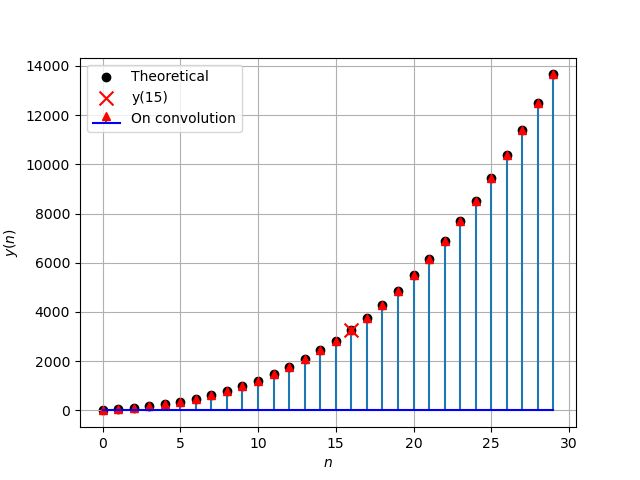
\includegraphics[width=\columnwidth]{ncert-maths/11/9/4/5/figs/plot.png}

\begin{center}
    \caption{Simulation v/s theoretical}
\end{center}
\end{figure}

